%
% File acl2020.tex
%
%% Based on the style files for ACL 2020, which were
%% Based on the style files for ACL 2018, NAACL 2018/19, which were
%% Based on the style files for ACL-2015, with some improvements
%%  taken from the NAACL-2016 style
%% Based on the style files for ACL-2014, which were, in turn,
%% based on ACL-2013, ACL-2012, ACL-2011, ACL-2010, ACL-IJCNLP-2009,
%% EACL-2009, IJCNLP-2008...
%% Based on the style files for EACL 2006 by 
%%e.agirre@ehu.es or Sergi.Balari@uab.es
%% and that of ACL 08 by Joakim Nivre and Noah Smith

\documentclass[11pt,a4paper]{article}
\usepackage[hyperref]{acl2020}
\usepackage{times}
\usepackage{graphicx}
\usepackage{latexsym}
\usepackage{fancyvrb}

\renewcommand{\UrlFont}{\ttfamily\small}

% This is not strictly necessary, and may be commented out,
% but it will improve the layout of the manuscript,
% and will typically save some space.
\usepackage{microtype}
\usepackage[natbib=false]{biblatex} 
\addbibresource{acl2020.bib}

\aclfinalcopy % Uncomment this line for the final submission
%\def\aclpaperid{***} %  Enter the acl Paper ID here

%\setlength\titlebox{5cm}
% You can expand the titlebox if you need extra space
% to show all the authors. Please do not make the titlebox
% smaller than 5cm (the original size); we will check this
% in the camera-ready version and ask you to change it back.

\newcommand\BibTeX{B\textsc{ib}\TeX}

\title{Stereo Reconstruction}

\author{Alex Rasla \\
  UC Santa Barbara \\
  \texttt{alexrasla@ucsb.edu}}

\date{February 2, 2022}

\begin{document}
\maketitle

\section{Algorithms}

In order to achieve a good stereo reconstruction, I first ensured I could find an appropriate 
 window size, compute the best raw sum of squared differences (SSD), and then generate a baseline disparity map. 
 Once I tested this baseline disparity generation on a variety of images, I decided to implement the Maximum Likelihood Stereo 
 Algorithm \cite{COX1996542}. This algorithm takes a Disparity Space Image (DSI) of a scanline between two stereo images and 
 uses dynamic programming to get the shortest path (lowest sum of dissimilarity scores) from the first to the last column. 
 Once this shortest path is calculated, we can choose to include occlusion filling to further increase the quality of the disparity maps.

\section{Data}

For this stereo reconstruction project, I used the 2006 Middlebury Stereo Dataset \cite{Hirschmller2007EvaluationOC}. 
 This dataset is a very trusted and standard dataset for stereo reconstruction algorithms because of its high-quality stereo 
 images and accurate ground truth disparity maps. Specifically, I utilized the Aloe, Cloth1, Rocks1, and Wood1 datasets for 
 both the full-size (1282x1110) and half-size (665x555) images.  Unfortunately, because it is very difficult and resource 
 dependent to generate accurate ground truth disparity maps, I was unable to create my own dataset to test my stereo reconstruction 
 algorithm.

\section{Libraries}

For this assignment, I used OpenCV, NumPy, and Numba. I used OpenCV to simply read and write images into memory, since my stereo matching algorithm did not require any feature matching or other low-level optimizations. Rather, it required a lot of pixel processing, computing formulas between windows, and matrix operations, all of which I used NumPy for. Furthermore, to speed up NumPy computation and vectorize the code, I used Numba, a high performance Python compiler that converts NumPy loops and dynamic programming into very fast machine code.

\section{Implementation Details}

In order to run this program, simply type the command: 
\begin{Verbatim}[fontsize=\small]
python3 stereo.py --dir [head directory of images] 
                  --left [left image] 
                  --right [right image] 
                  --out [output directory] 
                  --scale [disparity scale]
\end{Verbatim}
For this command, the --dir flag should be the head directory of images that contains subdirectories 
 with the downloaded/test datasets from Middlebury \cite{Hirschmller2007EvaluationOC}. The program goes 
 through all the subdirectories in --dir, gets right and left disparity images, saves left and right disparity 
 maps into the out folder in the subdirectory, and generates a bar graph of the Bad Matched Pixels (BMP)
  and timing of the different datasets. For the full-size images (1282x1110), the scale should be 1; for 
  half-size, the scale should be 2; for third-size, it should be 3.

\section{Results}

The results of my stereo reconstruction produced visually consistent disparity maps for all datasets, 
but produced slightly underwhelming results based on the BMP evaluation metric. 

$$BMP = \frac{1}{N} \sum_{(x, y)} (|d_{C}(x, y) - d_{T}(x, y)| > \delta_{d})$$

The BMP metric is a binary metric that checks whether a resultant disparity map is within a given $\delta$ value,
 and then computes the percentage of those that are within the value. In the original paper \cite{BMP}, the authors 
 chose a $\delta$ value of 1 to only allow a difference of 1 pixel between the generated disparity map and the ground 
 truth. In my evaluation, I focused on $\delta$ values of 5.
  % for left and right disparity images for each dataset and the time it took to calculate them.

My initial, basline attempt at generating disparity maps was simply using SSD. This disparity map was structurally accurate, 
 but evaluated to a BMP range of $0.55-0.76$ $(\delta = 5)$ for the left disparity maps. Next, to
 improve the BMP values and quality of the disparity maps, I used dyanmic programming without occlusion filling which significantly narrowed
 the BMP range to between $0.55-0.68$ for the left disparity maps ($\delta = 5$). Finally, when I added occlusion filling, this again improved the BMP value 
 to between $0.40-0.76$ ($\delta = 5$) for full-size and 0.52 and 0.67 ($\delta = 5$) for the half-size. Table \ref{tab:table1} gives a range of 
 BMP values given the size of images and a given delta value, figure \ref{fig:images} shows a visual comparison of the different disparity maps, 
 and figure \ref{fig:plots} shows a bar graph plot of the the different BMP values and the runtime to generate them.

 \begin{table}
    \centering
    \begin{tabular}{ |c|c|c|c| } 
     \hline
      & $\delta = 1$ & $\delta = 5$ & $\delta = 20$ \\
     \hline
     Full Size & 0.41-0.77 & 0.40-0.76 & 0.40-0.75\\ 
     \hline
     Half Size & 0.53-0.69 & 0.52-0.67 & 0.52-0.66\\ 
     \hline
    \end{tabular}
    \caption{The range of left image stereo reconstruction Bad Matched Pixel values for Dyanmic Programming with Occlusion}
    \label{tab:table1}
\end{table}

\begin{figure}
    \centering
    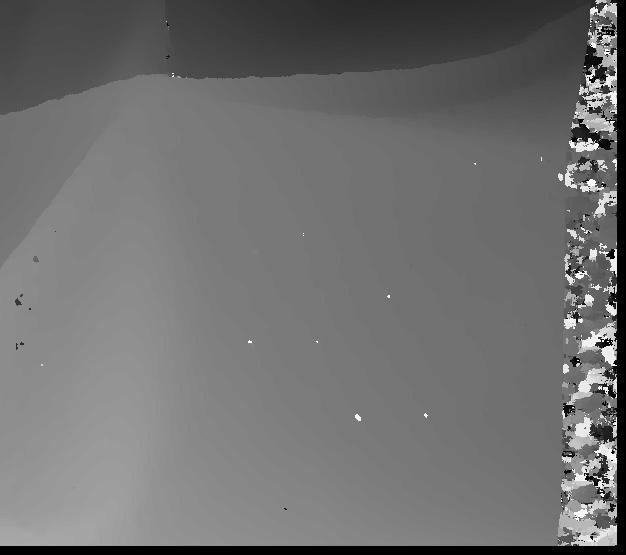
\includegraphics[width=0.13\textwidth]{figures/ssd_res5.png}
    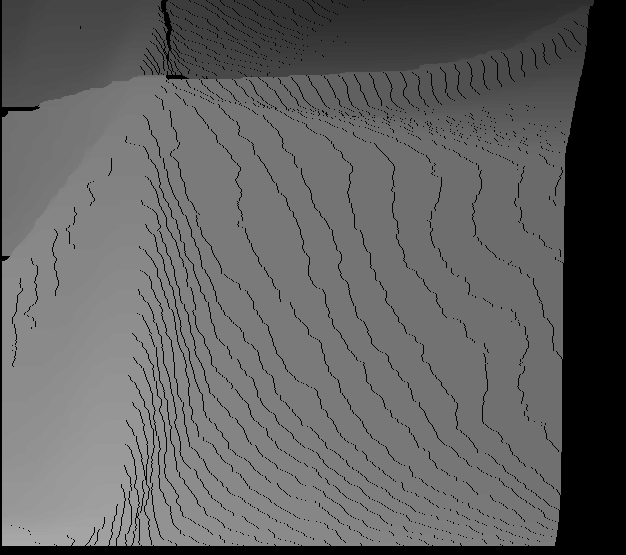
\includegraphics[width=0.13\textwidth]{figures/nofill_res5.png}
    
\includegraphics[width=0.13\textwidth]{figures/res5.png}
    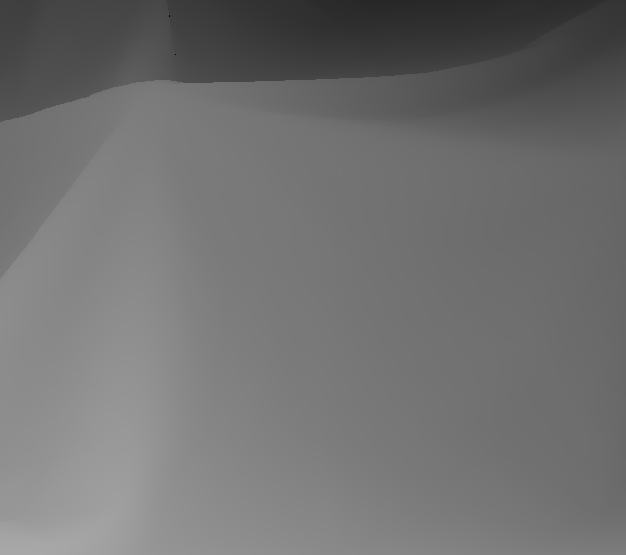
\includegraphics[width=0.21\textwidth]{figures/disp5.png}
    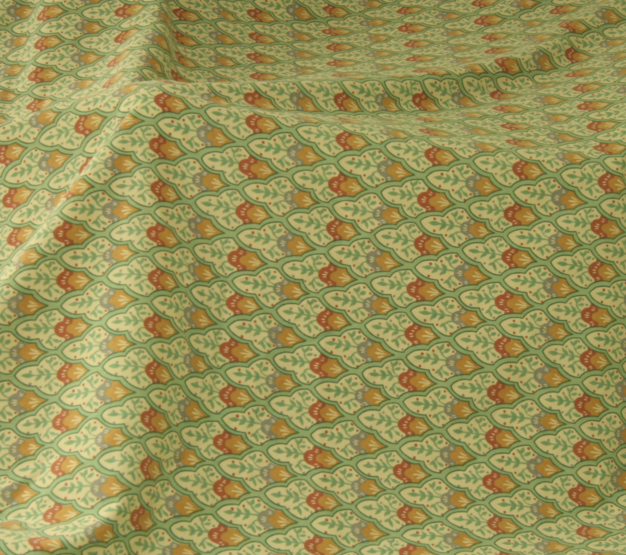
\includegraphics[width=0.21\textwidth]{figures/view5.png}
    \caption{The upper leftmost image is the raw SSD left disparity map for the Cloth1 full-size dataset; the upper middle is the result of dynamnic programming without occlusion; 
    the upper right is dynamic programming with occlusion; the lower left image is the ground truth; the lower right most is the original RGB image}
    \label{fig:images}
\end{figure}

\begin{figure}
  \centering
  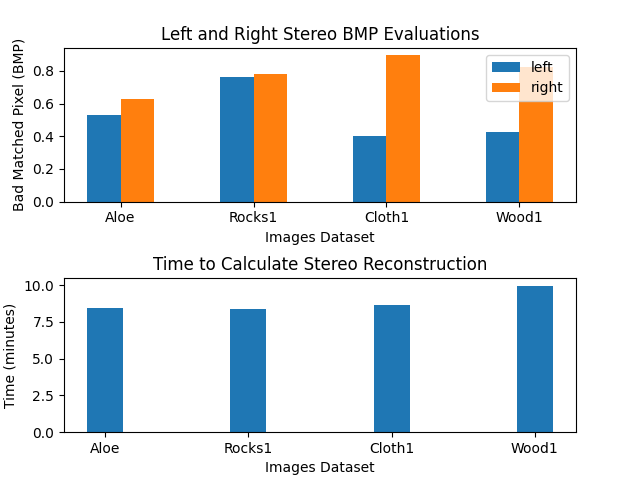
\includegraphics[width=0.45\textwidth]{figures/full_plots.png}
  \caption{A plot of the BMP score for the left and right disparity maps for full-size images in the Aloe, Rocks1, Cloth1, and Wood1 datasets}
  \label{fig:plots}
\end{figure}



\section{Discussion}

Throughout this project, I explored the difference between SSD disparity maps, dynamic programming disparity maps, 
 and dynamic programming with occlusion disparity maps. Because the latter two methods are built upon the typical SSD 
 scanline matching, I had to ensure the SSD was computed efficiently and quickly. To do this, I first used NumPy array 
 slicing to create a Disparity Space Image (DSI) between the left scanline and right scanline. This DSI gave me a MxM matrix, 
 where each value represented the SSD between a left pixel (row) and right pixel (column) on the scanline. Once this DSI was calculated, 
 to generate a simple SSD disparity map, I simply took the maximum values along each row to get the best matching (lowest SSD) 
 right pixel for every left pixel. 

To improve upon this and achieve a better result, I implemented the dynamic programming algorithm described in \cite{COX1996542}. 
 In order to implement this algorithm, it required an occlusion cost parameter which I found was best at 100,000. This occlusion 
 cost represents the cost to “occlude” a DSI matrix value, and proceed to the next value. This algorithm enhanced qualitative visual 
 accuracy of the raw SSD results by finding the shortest path on a particular scanline. Typically, I noticed that with an occlusion cost of any multiple of 100,000, 
 the BMP values increased. This makes sense because the shortest path algorithm relies on the occlusion cost to omit outlier pixels that have disparity values that 
 are too high. Also, if the cost is too low, we may end up with the same result as the SSD image. To further improve upon the dynamic programming algorithm, I implemented occlusion filling, which simply uses the disparity
 value of an adjacent pixel as opposed to giving it a grayscale value of 0. 
 
Alongside experimenting with the occlusion cost, I also experimented with the window size, and the magnitude of delta.
 With a bigger window size the runtime is around 2.5 times slower, and the BMP values increase significantly. When changing the
window size from 10 to 30, the the half-size images BMP range was $0.52-0.89$ ($\delta = 5$). For Cloth1 specifically, the BMP increased from 0.52 to 0.74. 
 When increasing the delta values even slightly, I expected the BMP values to decrease and lead to a better quantitative evaluation of the disparity images; however, as we can see in Table 
 \ref{tab:table1}, the change in $\delta$ values did not produce a signifcant change in BMP.  This is likely because the values 
 that lie outside of $\delta$ lie extremely far outside of $\delta$ and require $\delta$ values of at least a two orders of magnitude
 greater to effect the BMP score.

\printbibliography

\end{document}
